\chapter{Implementierug des Frameworks}

Dieses Kapitel beschäftigt sich mit der Architektur und Impelentierung des Framworks.
Das Framework schafft eine Abstraktionsebene für die Algorithmen, die die aktiven Topologien in den CEP-Systemem skalieren.
Das Framework soll ermöglichen, die einzelnen Komponenten in der Topologie zu skalieren. Die logische Struktur der Topologie wird dabei nicht verändert. Das vorliegende Modell ermöglicht die Steuerung mehrerer CEP-Topologien, welche auch über diverse CEP-Systeme verteilt werden können. 

\subsection{Architektur}

Die Architektur des Frameworks besteht aus mehreren logischen Komponenten und verfolgt zwei Ziele.
Eines der beiden Hauptziele der Architektur ist, dass das System einfach um weitere Algorithmen erweitert werden kann.
Um dieses Ziel zu erreichen, wurde eine Abstraktionsebene eingeführt, welche die Eigenschaften des realen CEP-Systems repräsentiert.
Diese Abstraktion wird durch ein Graphen-Modell repräsentiert, welches einen gerichteten, azyklischen Graphen modelliert.
Die implementierten Algorithmen arbeiten ausschließlich auf dem abstrahierten Modell.
Für die Implementation eines neuen Algorithmus, müssen nur die Daten aus dem Modell ausgelesen und anschließend verarbeitet werden.
Außerdem ist es möglich, mehrere Algorithmen für das gleiche Modell auszuführen um ihre Ergebnisse zu vergleichen.
Um einen Algorithmus für das System zu implementieren ist ausschließlich Wissen über das Modell notwendig.

Ein weiteres Ziel ist, dass das System für weitere CEP-Systeme außer Heron verwendet werden kann.
Dazu wurde eine API, die bereits in einer vorhergehenden Bachelorarbeit entwickelt wurde, erweitert.
Alle Komponenten des Systems benutzen diese API für die Kommunikation mit dem CEP-System, sodass diese alle system-spezifischen Befehle abstrahieren kann.
Die Seite der API, welche mit dem System direkt kommuniziert ist ein eigenständiger Adapter.
Dieser Adapter wird auf dem Rechner installiert, von dem das zu steuernde CEP-System kontrolliert wird.
Der Adapter ist über eine REST-API ansprechbar.
Somit kann das Framework auf einem eigenständigen Rechner installiert werden und das Zielsystem über die REST-Schnittstelle des Adapters kontrollieren.
Dies ermöglicht die Kontrolle von mehreren CEP-Systemen zur gleichen Zeit.
Eine Erweiterung des Frameworks für weitere Systeme über die Implementierung eines entspreche4nden Adapters zu erreichen.
Für die Erstellung eines neuen Adapters ist ausschließlich Wissen über die Spezifikation der REST-Schnittstelle notwendig.
Das Framework kann so über die REST-API verschiedene CEP-Systeme über eine einheitlichen Schnittstelle ansprechen.

Die Architektur des Systems ist in der Abbildung 5.1 dargestellt.
Im Folgenden werden die einzelnen Komponenten der Architektur genauer erläutert.

\begin{figure}
  \centering
  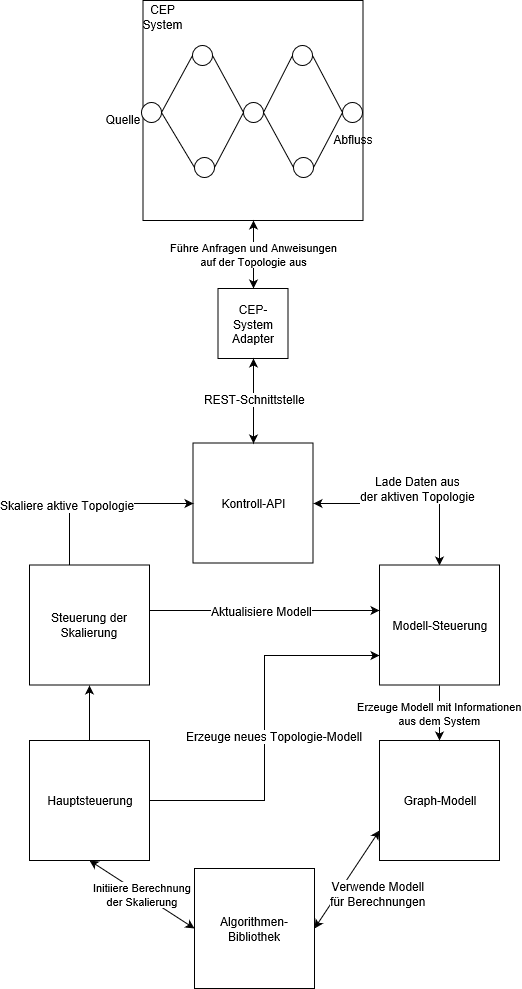
\includegraphics[width=\textwidth]{Systemaufbau.png}
  \caption{Architektur des Systems}
  \label{fig:Architektur}
\end{figure}

\section{Graph-Modell}
Das Graph-Modell repräsentiert die Topologie im realen CEP-System.
Alle Elemente der Topologie werden nach dem in Kapitel *********** vorgestellten Topologie-Modell abgebildet.
Es dient als Cache für Messdaten aus dem realen System.
Durch die Zwischenspeicherung wird ermöglicht, dass ein Modell eines bestimmten Zeitpunktes des realen Systems zur Verfügung gestellt werden kann. 
Würden die Algorithmen die Werte zur Laufzeit abfragen, also immer dann, wenn die Werte benötigt werden, kann dies zu einem inkonsistenten Modell führen.
Die Algorithmen verwenden das Modell, um die Inkosistenz von Messungen zu verschiedenen Zeitpunkten zu verhindern.

Jedes Modell besteht aus Pfaden und Operatoren.
Jeder Pfad stellt dabei eine geordnete Folge von Operatoren dar.
Das Modell erlaubt kreuzende Pfade, sodass Operatoren in mehreren Pfaden verwendet werden können.
Momentan kann im Modell keine selektive Weiterleitung der Tupel repräsentiert werden.
Dies bedeutet, dass ein Operator alle Tupel, die er versendet, an immer an alle folgenden Operatoren weiterleitet.
Operatoren sind über einen Namen identifizierbar und haben eine dem Parallelisierungsgrad entsprechende Anzahl an Tasks.
Sobald der Operator einen neuen Parallelisierungsgrad erhält, wird die entsprechende Anzahl Tasks gelöscht oder erzeugt.
Somit ist die Anzahl Tasks immer gleich dem Parallelisierungsgrad des Operators.
Der maximale und minimale Parallelisierungsgrad aller Operatoren kann über zwei Konstanten angegeben werden. 
Diese gelten für alle Operatoren in allen Modellen. 
Ein logisch schlüssiger Minimalwert ist der Parallelisierungsgrad 1.
Ein Parallelisierungsgrad kleiner als eins ist für einen aktiven Operator nicht gültig, da er keinen ausführenden Task besitzt.
Das Maximum kann entsprechend der Ressourcen, die im CEP-System zur Verfügung stehen, angepasst werden.
Pfade und Operatoren stellen die logische Struktur der Topologie dar.

Die ausführende Ebene, oder physische Struktur, wird durch Tasks und Kanäle repräsentiert.
Tasks sind die Recheninstanzen welche die Operation eines Operators auf Tupel ausführen.
In der vorliegenden Implementation des Graph-Modells ist die Zwischenspeicherung der Messwerte auf Task-Ebene vorgesehen.
Somit wird ermöglicht, dass ein detailliertes Modell der Topologie im CEP-System erzeugt werden kann.
Die ID der Tasks wird vom Operator automatisch erzeugt und wird aus dem Namen des Operators und einer fortlaufenden Nummer wie folgt gebildet: \textit{<Name>\_<Nummer>}.
Die niedrigste Nummer ist immer die eins.
Die höchste Nummer entspricht immer dem aktuellen Parallelisierungsgrad des Operators.
Für Tasks sind folgende Messwerte in der aktuellen Version des Modells vorgesehen:

\begin{itemize}
\item{Latenz des Tasks}
\item{Anzahl Ausführungen des Tasks}
\item{Anzahl eingehender Tupel}
\item{Anzahl ausgehender Tupel}
\item{Auslastung}
\item{Bearbeitungsdauer}
\item{Tupel-Ankunftsintervall}
\item{Varianz der Bearbeitungsdauer}
\item{Varianz des Tupel-Ankunftsintervalls}
\end{itemize}

Für die Messwerte der Tasks wird die Annahme getroffen, dass sie unabhängig vom Pfad sind.
Dies bedeutet zum Beispiel, dass alle eingehenden Tupel die selbe Bearbeitungsdauer benötigen.
Unabhängig davon von welchem vorhergehenden Operator sie stammen.
Alle für den Task erfassten Metriken differenzieren nicht die Herkunft der Tupel, sondern erfassen sie gesammelt.

Für viele Algorithmen wird nicht der Messwert eines einzelnen Tasks betrachtet, jedoch können die Werte gemittelt werden um einen aussagekräftigen Messwert für den gesamten Operator zu bekommen.

Die Kommunikation zwischen den Tasks wird durch die Kanäle repräsentiert.
Diese speichern Metriken der Kommunikationskanäle zwischen Tasks.
Für die Implementation des Modells wurde die Annahme getroffen, dass alle Tasks eines Operators mit allen Tasks der vorhergehenden und nachfolgenden Operatoren kommunizieren können.
Die Anzahl an Kanälen zwischen zwei Operatoren ist also das Produkt aus deren Parallelisierungsgraden.
Für Kanäle sind folgende Messwerte vorgesehen:

\begin{itemize}
\item{Latenz des Kanals}
\item{Latenz der Stapelverarbeitung}
\end{itemize}

Details zu den Messwerten werden in Kapitel ********* erläutert.

\section{Modell-Steuerung}

Die Modell-Steuerung erzeugt die Modellstruktur der Topologien und füllt diese anschließend mit Messwerten.
Alle Aktionen werden von der Hauptsteuerung initiiert.
Im ersten Schritt wird die Topologie vom CEP-System über die Kontroll-API ausgelesen.
Welche Topologie ausgelesen wird entscheidet die angegebene Adapteradresse.
Ein Adapter ist jeweils für eine Topologie zuständig.
Zuerst werden die Pfade der Topologie ausgelesen und im Graph-Modell die entsprechenden Operatoren und Pfade angelegt.
Dann wird der Parallelisierungsgrad der Operatoren gesetzt.
Diese erzeugen ,wie zuvor beschrieben, durch das setzen des Parallelisierungsgrades die entsprechende Anzahl an Tasks und Kanälen.

Anschließend erzeugt die Modell-Steuerung eine Zuweisung von Tasks im realen System zu den Tasks im Modell.
Die Tasks im Modell sind, wie im vorherigen Kapitel beschrieben, durchnummeriert und haben einen durch das Graph-Modell festgelegten Namen.
Diese Namen weichen sehr wahrscheinlich von den Namen im realen CEP-System ab.
Damit nun die Messwerte eines realen Tasks konsistent einem modellierten Task zugewiesen werden können, wird pro Operator eine Zuweisungstabelle für die Tasks erzeugt.
Diese Zuweisung muss mit jeder Änderung des Parallelisierungsgrades des Operators angepasst werden, da Tasks wegfallen oder hinzu kommen.
Ist die Zuweisung erfolgt werden zuletzt die Messwerte über die Kontroll-API in das Modell geladen.

\section{Steuerung der Skalierung}

Die Steuerung der Skalierung übernimmt zwei Aufgaben.
Zum Einen werden die Ergebnisse der ausgeführten Algorithmen an das CEP-System geben.
Dazu wird die Kontroll-API verwendet, der Adapter steuert die Anpassung der Parallelisierungsgrade in der aktiven Topologie.
Als Zweites wird nach erfolgreicher Anpassung der realen Topologie noch das Modell angepasst.
Hier werde ebenfalls die neuen Parallelisierungsgrade, welche die Algorithmen berechnet haben, gesetzt.

\section{Hauptsteuerung}

Die Hauptsteuerung ist die zentrale Steuereinheit des Frameworks.
Sie enthält die Logik, die die anderen Komponenten kontrolliert und die zuvor beschriebenen Abläufe steuert.
Sie instanziiert die anderen Komponenten für jede Topologie, die gesteuert werden soll.
Außerdem werden die Parameter definiert, die für Berechnungen in den Algorithmen verwendet werden.
Die zeitliche Abfolge aller Abläufe zu steuern ist die Kernaufgabe der Komponente.

\section{Kontroll-API}

Die Kontroll-API abstrahiert die APIs der verschiedenen CEP-Systeme.
Grundsätzlich besteht Sie aus zwei Teilen.
Ein Teil nimmt die Aufrufe aus dem Framework entgegen und wandelt sie in REST-Anfragen um.
Die Anfragen werden anschließend an den entsprechenden Adapter gesendet.
So wird die REST-Schnittstelle über die zur Verfügung gestellten Funktionen gekapselt.
Dieser Teil ist auf der gleichen Maschine wie die anderen Komponenten des Frameworks und wird direkt von den anderen Komponenten angesprochen.

Der zweite Teil, der Adapter, befindet sich auf der Maschine des zu steuernden CEP-Systems.
Er nimmt REST-Anfragen entgegen und setzt diese in Befehle für die API des CEP-Systems um.
Der Adapter ist somit der Teil, der die API des CEP-System auf eine einheitliche REST-Schnittstelle abstrahiert.
Außerdem kapselt der Adapter die zurückgelieferten Messwerte des CEP-Systems und vereinheitlicht sie für das Graph-Modell.
Deshalb ist die Implementation des Adapters essentiell für die Qualität des Graph-Modells.
Die Implementation des Adapters für das CEP-System Heron wird in Kapitel *********** ausführlich behandelt.

Die Kommunikation über die REST-API ermöglicht es, dass die beiden teile auf verschiedenen Maschinen installiert sein können.
Durch die Fern-Steuerung über die Schnittstelle können mit einer einzelnen Installation des Frameworks mehrere CEP-Systeme und Topologien gleichzeitig gesteuert werden.

\section{UML-Diagramm des Frameworks}



















